% DOCUMENT FORMAT ======================= -*- mode: LaTeX; coding: utf-8 -*- ===

\documentclass[diploma]{softlab-thesis}

% PACKAGE SETTINGS =============================================================

\usepackage{fontspec}
\usepackage{amsmath}
\usepackage{amsfonts}
\usepackage{multirow}
\usepackage{array}
\usepackage{mdwlist}
\usepackage{subfig}
\usepackage{floatrow}
\usepackage{float}
\usepackage{verbatim}
\usepackage{color}
\usepackage{graphicx}
\usepackage{xunicode}
\usepackage{xltxtra}
\usepackage{url}
%\usepackage{dsfont}
%\usepackage{microtype}
\usepackage{hyphenat}
\usepackage{multicol}
\usepackage{wrapfig}
\usepackage{lipsum}
\usepackage{listings}
\usepackage{paralist}
\usepackage{ulem}
\usepackage{tocvsec2}
\usepackage{url}
\usepackage[toc,page]{appendix}

\usepackage{epigraph}
\setlength\epigraphwidth{.5\textwidth}
% FONT SETTINGS ===============================================================

%\setromanfont[Mapping=tex-text]{CMU Serif}
%%\setromanfont[Mapping=tex-text]{CMU Sans Serif} % temporary change until printing
%%\setsansfont[Mapping=tex-text]{CMU Sans Serif}
%%\setmonofont[Mapping=tex-text]{CMU Typewriter Text}
%\setmainfont[Mapping=tex-text]{CMU Serif}
%%\setmainfont[Mapping=tex-text]{CMU Sans Serif}  % temporary change until printing

%\setromanfont[Mapping=tex-text,ExternalLocation=fonts/]{cmunrm.otf}
%\setsansfont[Mapping=tex-text,ExternalLocation=fonts/]{cmunss.otf}
%\setmonofont[Mapping=tex-text,ExternalLocation=fonts/]{cmuntt.otf}
%\setmainfont[Mapping=tex-text, ExternalLocation=fonts/]{cmunss.otf}

\defaultfontfeatures{Mapping=tex-text}
%\setromanfont{Linux Libertine O}
\setromanfont{DroidSerif}

% CUSTOM COLORS ===============================================================

\definecolor{gray}{rgb}{0.5,0.5,0.5}
\definecolor{darkgreen}{rgb}{0.0,0.5,0.0}
\definecolor{mygreen}{rgb}{0,0.6,0}
\definecolor{mygray}{rgb}{0.5,0.5,0.5}
\definecolor{mymauve}{rgb}{0.58,0,0.82}
\definecolor{myorange}{RGB}{246,177,50}

% CUSTOM COMMANDS =============================================================

\newcommand\fixme{\textrm{\textbf{\textcolor{red}{FIXME: }}}}
\newcommand\todo{\textrm{\textbf{\textcolor{myorange}{TODO: }}}}
\newcommand\mytilde{\raise.17ex\hbox{$\scriptstyle\sim$}}
\newcommand\okeanos{\textbf{\raise.17ex\hbox{$\scriptstyle\sim$}okeanos }}


% Layout macros
\newcommand\spa[1]{\; #1 \;}

% Font macros
\newcommand\resfont[1]{\ensuremath{\mathtt{#1}}}

% Mathematical macros
\newcommand\setmap[3]{#1\{#2 \mapsto #3\}}
\newcommand\getmap[3]{(#2 \mapsto #3) \in #1}
\newcommand\tuple[2]{\ensuremath{\langle#1, #2\rangle}}
\newcommand\mfrac[2]{\ensuremath{\dfrac{#1}{#2}}}
\newcommand\nequiv[2]{\ensuremath{#1 \not\equiv #2}}

% Core Ruby Operational Semantics letter bindings
\newcommand\mem{\mu}

% Core Ruby Operational Semantics low level macros
\newcommand\state[2]{(#1, #2)}
\newcommand\transition[1]{\ensuremath{\overset{#1, c*}{\rightarrow}}}
\newcommand\range[2]{#1, ..., #2}
\newcommand\midrange[5]{\range{#1}{#2}, #3, \range{#4}{#5}}

% Core Ruby Operational Semantics high level macros
\newcommand\operation[5]{\ensuremath{\state{#1}{#2} \transition{#3} \state{#4}{#5}}}
\newcommand\propagation[2]{\operation{#1}{\mem}{#2}{#1'}{\mem'}}

% Core Ruby specific Operational Semantics macros
\newcommand\semicolon[2]{#1; \; #2}
\newcommand\assign[2]{#1 = #2}
\newcommand\mcall[3]{#1.\texttt{#2}(#3)}
\newcommand\ifte[3]{\resfont{if} \; #1 \; \resfont{then} \; #2 \; \resfont{else} \; #3}
\newcommand\newclass[2]{#1.\resfont{new}(#2)}
\newcommand\methoddef[3]{\resfont{def} \; #1(#2) = #3}
\newcommand\classdef[2]{\resfont{class} \; #1 = #2}
\newcommand\with[3]{with \; \tuple{#1}{#2} \; do \; #3}

% Success Typing macros
\newcommand\ssub{\sqsubseteq\_S}

% Core Ruby Success Typing letter bindings
\newcommand\classlist{\Delta}
\newcommand\envir{\Gamma}
\newcommand\fields{\Phi}
\newcommand\currclass{l}

% Core Ruby Success Typing inferencing macros
\newcommand\stinfer[5]{\classlist; \; #1; \; \fields \; \underset{\currclass}{\vdash} \; #2: #3 \; \& \; #4; \; #5}


%%%%%%%%%%%%%%%%%%%%%%%%%%% CACHED STUFF %%%%%%%%%%%%%%%%%%%%%%%%%%%

\newcommand\xcache{\texttt{xcache} }

%%%%%%%%%%%%%%%%%%%%%%%%%%% HASKELL STUFF %%%%%%%%%%%%%%%%%%%%%%%%%%%

%\newcommand\typerep[1]{\ensuremath{#1}}
\newcommand\typerep[1]{\lstinline[basicstyle=\normalsize\ttfamily,keywords={}]|#1|}
\newcommand\typefootrep[1]{\textbf{\lstinline[basicstyle=\footnotesize\ttfamily,keywords={}]|#1|}}
% \newcommand\ttyperep[1]{\typerep{#1}}
% \newcommand\mtyperep[1]{\mbox{\typerep{#1}}}

% Arrow types
\newcommand\typeto[2]{\typerep{#1} \typerep{->} \typerep{#2}}
\newcommand\typetotwo[3]{\ensuremath{\typerep{#1} \typerep{->}
	\typerep{#2} \typerep{->}
	\typerep{#3}}}

\newcommand\tyconapone[2]{\ensuremath{\mbox{\typerep{#1}} \:\: \mbox{#2}}}
\newcommand\tyconaponeC[2]{\ensuremath{\mbox{\typerep{#1}} \:\: \mbox{\typerep{#2}}}}
% \newcommand\tyconapone[2]{\typerep{#1} $\:$ \typerep{#2}}

\newcommand\tyconaptwo[3]{\ensuremath{\mbox{\typerep{#1}} \:\: \mbox{#2} \:\: \mbox{#3}}}


% FIGURE SETUP ===============================================================

\newcommand\diagram[2]{
\begin{figure}[h!]
	\centering
	\includegraphics[width=\textwidth,height=\textheight,keepaspectratio]
	{diagrams/#2}
	\caption{#1}
	\label{fig:#2}
\end{figure}
}

\newcommand\diagramscale[3]{
\begin{figure}[h!]
	\centering
	\includegraphics[scale={#3}]
	{diagrams/#2}
	\caption{#1}
	\label{fig:#2}
\end{figure}
}
\newcommand\diagramstrict[2]{
\begin{figure}[H]
	\centering
	\includegraphics[keepaspectratio]
	{diagrams/#2}
	\caption{#1}
	\label{fig:#2}
\end{figure}
}


% SPELLING =====================================================================

% CODE HIGHLIGHTING ============================================================

% Define common settings for code listings

\lstset{
backgroundcolor=\color{white},
basicstyle=\small\ttfamily,		% style for code
breakatwhitespace=false,        % sets if automatic breaks should only
% happen at whitespace
breaklines=true,                % sets automatic line breaking
captionpos=b,                   % sets the caption-position to bottom
commentstyle=\color{mygreen},   % style for comments
escapeinside={\%*}{*)},         % if you want to add LaTeX within your code
frame=single,                   % adds a frame around the code
keepspaces=true,                % keeps spaces in text, useful for
%keywordstyle=\color{blue}\bfseries,
% keyword style
numbers=left,
numbersep=5pt,                  % how far the line-numbers are from the
% code
numberstyle=\tiny\color{mygray},% style for line-numbers
rulecolor=\color{black},
stepnumber=1,                   % the step between two line-numbers. If
% it's 1, each line will be numbered
stringstyle=\color{mymauve},    % style for strings
tabsize=2,                      % sets default tabsize to 2 spaces
}

\lstdefinestyle{plain}
{
stepnumber=0
}

% Create new commands for simpler usage

\newcommand\plaintext[2]{
\lstinputlisting[style=plain, caption={#1},
label=lst:#2]{src/#2}
}

% CHANGE MATH FONT ============================================================

% HYPERREF MUST BE LAST =======================================================

\usepackage[xetex,colorlinks=true,linkcolor=blue,citecolor=darkgreen]{hyperref}

% DOCUMENT INFORMATION =========================================================

\title{Δημιουργία εργαλέιου για επιθέσεις σε συμπιεσμένα, κρυπτογραφημένα πρωτόκολλα}

% ===============> FIXME
\author{Σαραφιανού Ευδοξία}
\authoren{Sarafianou Evdoxia}
\datedefense{23}{1}{2017}
\supervisor{Αριστείδης Παγουρτζής}
\supervisorpos{Αναπληρωτής Καθηγητής ΕΜΠ}
\committeeone{Αριστείδης Παγουρτζής}
\committeeonepos{Αναπληρωτής Καθηγητής ΕΜΠ}
\committeetwo{Δημήτριος Φωτάκης}
\committeetwopos{Επίκουρος Καθηγητής ΕΜΠ}
\committeethree{Άγγελος Κιαγιάς}
\committeethreepos{Επίκουρος Καθηγητής ΕΚΠΑ}
\hypersetup{
pdftitle={},
pdfauthor={test},
pdfsubject={},
pdfkeywords={}
}


% MAIN DOCUMENT ================================================================

\begin{document}

\frontmatter
\maketitle

\def\templen{\parindent}
\setlength{\parindent}{0pt}
\setlength{\parskip}{1.5ex plus 0.5ex minus 0.2ex}

\begin{abstractgr}

Η ασφάλεια είναι ένα από τα βασικά χαρακτηριστικά κάθε υπολογιστικού
συστήματος, καθώς εξασφαλίζει την εμπιστευτικότητα, την ακεραιότητα και τη διαθεσιμότητα
της πληροφορίας. Η παρούσα εργασία ερευνά επιθέσεις πάνω σε συμπιεσμένα
κρυπτογραφημένα πρωτόκολλα και συγκεκριμένα αναπτυσει περαιτερω την επίθεση BREACH.

Προτινονται στατιστικές μέθοδοι που επιτρεπουν να πραγματοποιηθεί
η επίθεση σε πραγματικες ιστοσελίδες που χρησιμοποιουν συγχρονες κρυπτογραφικες
τεχνικες. Επιπλεον, αναπτυχθηκαν τεχικές βελτιστοποίησης της επίθεσης που συντομεύουν
την επιθέση εως και 500 φορές σε θεωρητικό επίπεδο.

Δημηιουργήσαμε ένα εργαλειο, το Rupture, που εφαρμόζει τις στατιστικές μας μεθόδους και
τις τεχνικές βελτιστοποίησης. Το Rupture ειναι γραμμενο σε κωδικα επιπέδου παραγωγής 
ελευθερου λογισμικού και αυτοματοποιει την επιθεση. 
Το RESTful API που εκθέτει σε συνδυασμό με το Web User Interface το καθιστούν
ένα εύχρηστο εργαλείο που επιτρέπει στους επιτιθέμενους να πραγματοποιούν μαζικές 
επιθέσεις.

Η δημιουργία αυτού του εργαλείου δε στοχεύει σε καμία περίπτωση σε κακόβουλη χρήση.
Αντίθετα, επιδιώκει να ευαισθητοποιήσει την κοινότητα για τις επιθέσεις σε συμπιεσμένα
κρυπτογραφημένα πρωτόκολλα. Αυτες οι επιθέσεις ειναι αρκετα εκλεπτυσμένες, με αποτέλεσμα
να θεωρείται αμφίβολο το αν μπορούν να πραγματοποιηθούν σε πραγματικές επιθέσεις. 

Η δημίουργια του Rupture ειναι συνεργατικη με τους (αλφαβητική σειρά): Δημήτρη Γρηγορίου, 
Δημήτρη Καρακώστα, Διονύση Ζήνδρο.
Ανανεωμένες εκδόσεις της παρούσας εργασίας μπορούν να βρεθούν στον ακόλουθο
σύνδεσμο: \url{https://github.com/esarafianou/rupture-thesis}. Το εργαλείο
Rupture βρίσκεται στο σύνδεσμο:\url{https://github.com/dionyziz/rupture}.

\end{abstractgr}

\begin{abstracten}

Security is a fundamental aspect of every computer system. as it reassures
 confidentiallity, integrity and availability of the data. This work investigates
attacks on compressed encrypted protocols, and develops further the BREACH attack.

New statistical methods are being proposed, which allow the attack to perform in reallife websites
which use the latest cryptographic techniques. New optimizations of the attack were also developed, which speed
up the attack up to 500 times in the theoretical model.

We implemented a framework,Rupture, which applies our statistical methods and 
optimization techniques. Rupture is open-source, production level and automates the attack.
The RESTful API it exposes in combination with the Web User Interface make it an easy-to-use tool 
which allows the attackers to perform attacks in the wild.

The implementation of this framework focuses by no means in malicious purposes. On the contrary,
it aims to sensitize the community aboot compression side-channel attacks. Such attacks are quite 
sophisticated and the community doubts whether the could be reallife attacks

Rupture is a collaborative work with (alphabetical order): Dimitris Grigorioy, Dimitris Karakostas
and Dionysis Zindros.

Updated versions on the current work can be found on the following link:
\url{https://github.com/esarafianou/rupture-thesis}. Ruptre repository is:
\url{https://github.com/dionyziz/rupture}

\end{abstracten}

\begin{acknowledgementsgr}
Η παρούσα διπλωματική εργασία εκπονήθηκε στα πλαίσια της φοίτησής μου στο τμήμα
Ηλεκτρολόγων Μηχανικών και Μηχανικών Υπολογιστών του Εθνικού Μετσόβιου
Πολυτεχνείου.

Η διπλωματική αυτή εκπονήθηκε υπό την επίβλεψη του καθηγητή Αριστείδη Παγουρτζή,
τον οποίο θα ήθελα να ευχαριστήσω θερμά για τη βοήθειά του, καθώς και για το
γεγονός ότι μέσω της διδασκαλίας της Κρυπτογραφίας με εισήγαγε
και μου ενεπνευσε την αγαπη για το αντικείμενο.

Ακόμα, θα ήθελα να ευχαριστήσω τον Διονύση Ζήνδρο, για την αμέριστη βοηθεια και καθοδηγηση του
στο επίπεδο της εκπόνησης της εργασιας, τον Δημήτρη Καρακώστα για τις συμβουλές και
τις διορθώσεις του στον κώδικα καθώς και τον Πέτρο Αγγελάτο για την πρακτική και συναισθηματική υποστήριξή του.

Τέλος, θα ήθελα να ευχαριστήσω τους φίλους και την οικογένειά μου για τη στήριξη
που μου παρείχαν όλα αυτά τα χρόνια.

\end{acknowledgementsgr}

\setlength{\parindent}{\templen}
\setlength{\parskip}{0pt}
\tableofcontents
\listoffigures
%\listoftables
\renewcommand{\lstlistlistingname}{List of Listings}
\lstlistoflistings % changed the title above

\mainmatter
% moved these two commands here so that they don't influence the toc
\setlength{\parindent}{0pt}
\setlength{\parskip}{1.5ex plus 0.5ex minus 0.2ex}

\renewcommand\floatpagefraction{.7}

\chapter{Εισαγωγή}\label{ch:intro}

\section{Εισαγωγή}\label{sec:intro}

Τα τελευταία χρόνια παρατηρείται μια αύξηση του ενδιαφέροντος της κοινωνίας
σχετικά με τα θέματα της ασφάλειας και της ιδιωτικότητας της πληροφορίας στο
Διαδίκτυο. Οι αποκαλύψεις του Snowden, η διαρροή προσωπικών στοιχείων και
κωδικών χρηστών μεγάλων εταιρειών, όπως yahoo και dropbox άλλαξαν τον τρόπο
με τον οποίο αντιλαμβα-νόμαστε τη χρήση online υπηρεσιών. Οι ερευνητές και
χρήστες στράφηκαν στην αναζήτηση λύσεων ώστε οι επικοινωνίες να γίνουν πιο
ασφαλείς απέναντι σε κάθε είδους αντιπάλους.

Στην παρούσα εργασία στοχεύουμε να αναδείξουμε αδυναμίες στα πρωτόκολλα
που χρησιμοποιούνται στο διαδίκτυο και μέσω της δημοσιευσής της να 
ευαισθητοποιήσουμε την κοινότητα ώστε να αντιμετωπιστούν αποτελεσματικά αυτές
οι ευπάθειες.

Η έρευνά μας επικεντρώνεται σε επιθέσεις ενάντια σε πρωτόκολλά συμπίεσης που
εφαρμόζονται στα δεδομένα πριν την κρυπτογράφηση και μεταφορά τους. Συγκεκριμένα,
επεκτείνουμε υπάρχοντα μοντέλα επίθεσης, όπως το BREACH και δημιουργούμε ένα εργαλείο
που πραγματοποιεί με αυτοματοποιημένο τρόπο τέτοιες επιθέσεις.

Το λογισμικό συμπίεσης στο οποίο επικεντρωθήκαμε είναι το gzip, που 
χρησιμοποιείται ευρέως στο Διαδίκτυο. Το gzip εφαρμόζει τον αλγόριθμο
DREFLATE, που αποτελεί τον συνδυασμό των άλγορίθμων συμπίεσης Huffman
και LZ77. Η επίθεση που επεκτείνουμε εκμεταλλεύεται τον τρόπο με τον
οποίο συμπιέζει κείμενα το LZ77 ενώ αντίθετα ο αλγόριθμος Huffman
δυσκολεύει την επίθεση.

Το πιο διαδεδομένο πρωτόκολλο μεταφοράς δεδομένων στο Διαδίκτυο είναι το
HTTP (Hyper-Text-Transfer Protocol). Τα δεδομένα που μεταφέρονται μέσω HTTTP
δεν είναι κρυπτογρα-φημένα, με αποτέλεσμα οποιοσδήποτε επιτειθέμενος ελέγχει
το δίκτυο μας, να μπορει να διαβάσει και να αλλοιώσει τα δεδομενα που μεταφέρονται.
Η εξέλιση του HTTP, το HTTPS καλύπτει αυτό το κενό στην ασφάλεια με την εισαγωγή
ενός ακόμα επιπέδου δικτύου πριν το επίπεδο εφαρμογής που αρχικά ήταν το SSL 
(Secure Socket Layer) και στη συνέχεια το TLS (Transport Layer Security). Το επίπεδο αυτό
επιβάλλει την κρυπτογράφηση των δεδομένων πριν  απο τη μεταφορά του και εγγυάται
έτσι την εμπιστευτικότητα, ακεραιότητα και διαθεσιμότητα των δεδομένων.

Οι αλγόριθμοι κρυτπογράφησης που χρησιμοποιούνται σ' αυτό το επίπεδο μπορούν να
χωριστούν σε δύο μεγάλες κατηγορίες: αλγόριθμοι ροής και αλγόριθμοι δέσμης.
Στην πρώτη περίπτωση, τα δεδομένα κρυπτογραφούνται ως μια συνεχής ροή,  ενώ στη 
δεύτερη περίπτωση χωρίζονται σε δέσμες ίσου μεγέθους και κρυπτογραφείται κάθε δέσμη χωριστά. 
Σε περίπτωση που τα δεδομένα δεν κατανέμονται με ακρίβεια σε δέσμες, εισάγεται τεχνητός
θόρυβος ώστε να επιτευχθεί το επιθυμητό μέγεθος και να ευθυγραμμιστεί η κάθε δέσμη.

Ο κυριότερος αλγόριθμος ροής ειναι ο RC4, ο οποίος όμως δεν χρησιμοποιείται πλέον
γιατι εχουν βρεθει σημαντικές ευπάθειες του που τον καθιστούν ανασφαλή. Ο πιο
διαδεδομένος αλγόριθμος δέσμης ειναι ο AES, που με διάφορες παραλλαγές είναι ο
πιο ευρέως χρησιμοποιούμενος αλγόριθμος κρυπτογράφησης. Αν και οι αλγόριθμοι ροης
καθιστούν την επίθεση που περιγράφουμε αρκετά εύκολη, με την παρούσα εργασία
καταδεικνύουμε οτι οι αλγόριθμοι δέσμης όπως ο AES δε μας προστατεύουν απόλυτα από
τέτοιες επιθέσεις. 

Προκειμένου να πετύχουμε την επίθεση στον αλγόριθμο AES χρησιμοποιήσαμε στατιστικές
μεθόδους και τεχνητό θόρυβο για να ξεπεράσουμε τις δυσκολίες που εισαγονται από τη
χρήση δεσμών. Ταυτόχρονα εισήγαγαμε τεχνικές που βελτιστοποιούν την απόδοση της
επίθεσης και μας επιτρέπουν να την πραγματοποιούμε σε πραγματικό χρόνο.

Αναπτύξαμε ανοιχτό λογισμικό σε κώδικα επιπέδου παραγωγής που εφαρμόζει τις στατιστικές
μεθόδους και τεχνικές βελτιστοποίησης μας. Το λογισμικό είναι ενα service-based σύστημα
αρχιτεκτονικής που αυτοματοποιεί την επίθεση καθώς απαιτεί μικρή διαμόρφωση πριν από την
επίθεση. Δίνει τη δυνατότητα για πολλαπλές επιθέσεις την ίδια στιγμή σε διαφορετικά θύματα
και ιστοσελίδες. Με το λογισμικό αυτό, πραγματοποιήσαμε επιθεσεις σε εργαστηριακές ιστοσελίδες.

Όσον αφορά τις στατιστικές μεθόδους, η χρήση πιθανοτητων στην επίθεση μας την καθιστά μη
ντιτερμινιστική. Προκειμένου λοιπόν να έχουμε ακρίβεια στα αποτελέσματα μας, έχουμε εισάγει
μια μετρική που εκφραζει την αυτοπεποιθησή μας για τα αποτελέσματα που παραγονται απο
τις στατιστικές μας μεθόδους. Μόνο αν αυτή ειναι ικανή, θεωρούνται έγκυρα τα δεδόμένα μας.
Σε διαφορετική περίπτωση, απορρίπτονται.


Εν κατακλείδι, η παρούσα εργασία αποτελεί τη συνέχεια μια ομάδας ερευνών που
παρουσιάστηκαν τα τελευταία χρόνια και φανέρωσαν βασικές αδυναμίες στα
συστήματα που χρησιμοποιούμε κατά κόρον. Είναι σημαντικό να επεκταθεί με νέες
τεχνικές βελτιστοποίησης της επίθεσης και, κυρίως, νέες μεθόδους αντιμετώπισής
της.

\section{Δομή της εργασίας}\label{sec:structure}

Η εργασία έχει δομηθεί ως εξής:

 
\begin{description} \item{Κεφάλαιο \ref{background}} \hfill \\

Το κεφάλαιο αυτό παρέχει στον αναγνώστη βασικές πληροφορίες, τόσο σε τεχνικό όσο
και σε θεωρητικό επίπεδο, οι οποίες θα χρησιμοποιηθούν στη συνέχεια.
Θα περιγράψουμε τους πιο διαδεδομένους αλγόριθμους συμπίεσης, καθώς και βασικά
πρωτόκολλα που χρησιμοποιούνται για την ασφάλεια στις επικοινωνίες, καθώς και
επιθέσεις εναντίων τους.\hfill \\

\item{Κεφάλαιο \ref{statistic_methods}} \hfill \\
 
Το κεφάλαιο αυτό εισαγει στατιστικές μεθόδους για να παρακαμφθουν εμπόδια
και να γίνει δυνατή η επίθεση σε αλγόριθμους δέσμης. Προτίνονται ακόμα μέθoδοι
βελτιστοποίησης που αυξάνουν την ταχύτητα και την απόδοση της επίθεσης.


\item{Κεφάλαιο \ref{rupture}} \hfill \\

Σ' αυτο το κεφάλαιο περιγράφουμε το εργαλείο που δημιουργήσαμε για επιιθέσεις
σε συμπιεσμένα κρυπτογραφημένα πρωτόκολλα. Συγκεκριμένα, επισημαίνουμε τις
προυποθέσεις κατω απ τις οποίες πραγματοποιείται μια τέτοια επίθεση, αναλύουμε
την ορολογία που χρησιμοποιείται στο εργαλειο και περιγραφουμε διεξοδικα τα
διαφορα μέρη του και τις λειτουργίες που αυτά επιτελούν.


\item{Κεφάλαιο \ref{rupture_api}} \hfill \\

Το κεφάλαιο αυτό περιγράφει πως επεκτείναμε το εργαλείο μας ώστε να γίνει πιο
λειτουργικό και εύχρηστο. Περιγράφει το RESTful API που δημιουργήσαμε και τις
κλήσεις που γίνονται σ'αυτο καθώς και τη λειτουργικότητα της διεπαφής χρήστη
(User Interface).


\item{Κεφάλαιο \ref{appendix}} \hfill \\

Ο κώδικας υλοποίησης της επίθεσης.  

\end{description}


\chapter{Theoretical background}\label{background}

In this chapter, we intend to provide the necessary background to the user
to understand the mechanisms used later in the work. The description of
each system is only a short introduction to familiarize the reader with
the needed concepts.

Specifically, section \ref{sec:gzip} describes the functionality of the gzip
compression software and the algorithms that it entails. Section
\ref{sec:sameorigin} covers the same-origin policy that applies in the web
application security model. In section \ref{sec:tls} we explain Transport
Layer Security, which is the widely used protocol that provides communications
security over the Internet. Finally, in section \ref{sec:mitm} we describe
attack methodologies, such as ARP spoofing, in order for an
adversary to perform a Man-in-the-Middle attack.

\section{gzip}\label{sec:gzip}

gzip is a file format and a software application used for file compression and
decompression. It is the most popular compression method on the Internet, integrated
into protocols such as HTTP and XMPP. Derivatives of gzip include the tar utility, which 
can extract .tar.gz files, as well as zlib, an abstraction of the DEFLATE algorithm in 
library form.\footnote{\url{https://en.wikipedia.org/wiki/Gzip}}

It is based on the DEFLATE algorithm, which is a composition of LZ77 and Huffman
coding. DEFLATE could be described in short by the following compression schema:

\begin{math}DEFLATE(m) = Huffman(LZ77(m))\end{math}

In the following sections we will briefly describe the functionality of both
these compression algorithms.

\subsection{LZ77}\label{subsec:lz77}

LZ77 is a lossless data compression algorithm published by A. Lempel and J. Ziv
in 1977 \cite{lz77}. It achieves compression by replacing repeated occurrences 
of data with references to a single copy of that data existing earlier in the 
uncompressed data stream. A match is encoded by a pair of numbers called a 
length-distance pair, the first of which represents the length of the repeated
portion and the second of which describes the distance backwards in the stream.
In order to spot repeats, the protocol needs to keep track of some amount of the
most recent data, specifically the latest 32 kilobytes. This data is held in a
sliding window, the initial appearance of a portion of data needs to have occurred
at most 32 Kb up the data stream, in order to be compressed. Also, the minimum
length of a text that can be compressed is 3 characters. Compressed text can
refer to literals as well as pointers.

Below you can see an example of a step-by-step execution of the algorithm for a
chosen text:

\begin{figure}[H] \caption{Step 1: Plaintext to be compressed} \centering
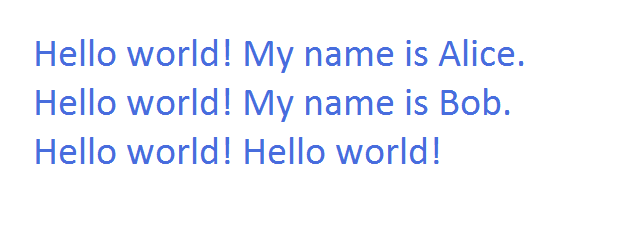
\includegraphics[width=0.5\textwidth]{diagrams/lz77_1.png}\end{figure}
\begin{figure}[H] \caption{Step 2: Compression starts with literal
representation} \centering
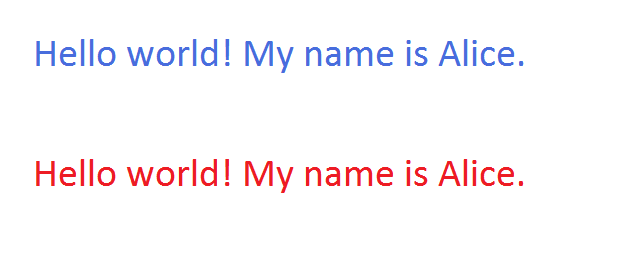
\includegraphics[width=0.35\textwidth]{diagrams/lz77_2.png}\end{figure}
\begin{figure}[H] \caption{Step 3: Use a pointer at distance 31 and length 25}
\centering
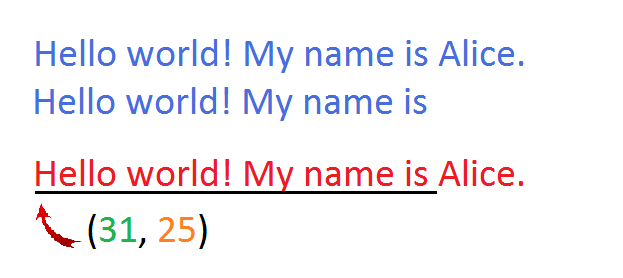
\includegraphics[width=0.35\textwidth]{diagrams/lz77_3.png}\end{figure}
\begin{figure}[H] \caption{Step 4: Continue with literal} \centering
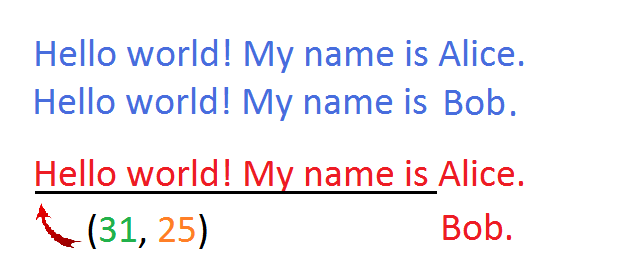
\includegraphics[width=0.35\textwidth]{diagrams/lz77_4.png}\end{figure}
\begin{figure}[H] \caption{Step 5: Use a pointer pointing to a pointer}
\centering
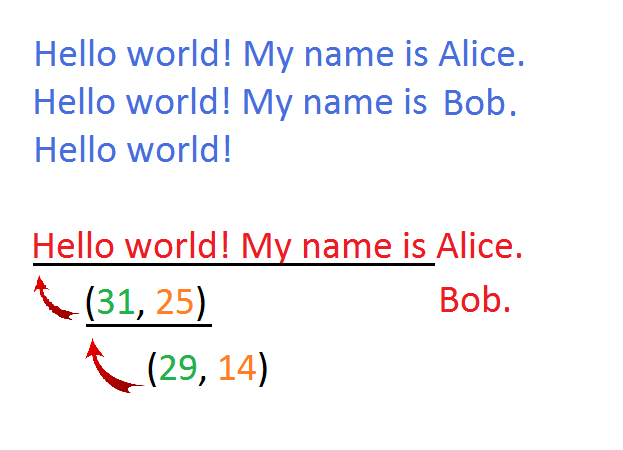
\includegraphics[width=0.35\textwidth]{diagrams/lz77_5.png}\end{figure}
\begin{figure}[H] \caption{Step 6: Use a pointer pointing to a pointer pointing
to a pointer} \centering
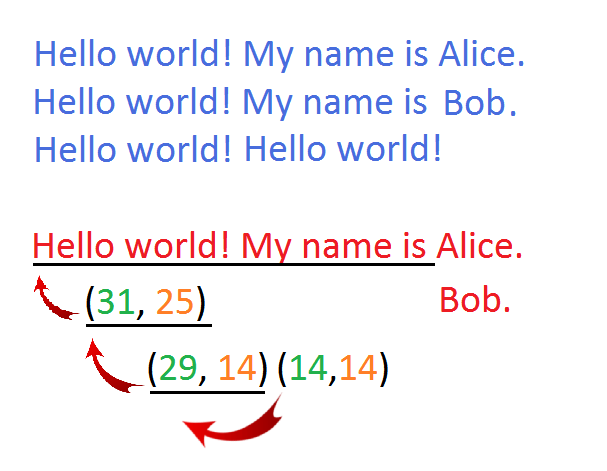
\includegraphics[width=0.35\textwidth]{diagrams/lz77_6.png}\end{figure}


\subsection{Huffman coding}\label{subsec:huffman}

Huffman coding is also a lossless data compression algorithm developed by David
A. Huffman and published in 1952 \cite{huffman}. When compressing a text with
this algorithm, a variable-length code table is created to map source symbols to
bit streams. Each source symbol can be represented with less or more bits
compared to the uncompressed stream, so the mapping table is used to translate
source symbols into bit streams during compression and vice versa during
decompression. The mapping table could be represented as a binary tree of nodes,
where each leaf node represents a source symbol, which can be accessed from the 
root of the tree by following the left path for 0 and the right path for 1. Each
source symbol can be represented only by leaf nodes, therefore the code is
prefix-free, i.e. no bit stream representing a source symbol can be the prefix
of any other bit stream representing a different source symbol. The final
mapping of source symbols to bit streams is calculated by finding the frequency
of appearance of each source symbol of the plaintext. That way, most common
symbols will be coded in shorter bit streams, resulting in a compression of the 
initial text. Finally, the compression mapping needs to be included in the final
compressed text so that it can be used during decompression.

Below follows an example of a plaintext and a valid Huffman tree that can be
used for compressing it:

\bigskip \centerline{\textit{\textbf{Would a helium balloon float on the moon?}}}

\bigskip \centerline{\textbf{Frequency Analysis}}

\begin{table}[H] \centering \begin{tabular}{ | l | l | l | l | } \hline
\textbf{o}: 7 & \textbf{l}: 5 & \textbf{a}: 3 & \textbf{n}: 3 \\ \textbf{u}: 2 &
\textbf{h}: 2 & \textbf{e}: 2 & \textbf{m}: 2 \\ \textbf{t}: 2 & \textbf{w}: 1 &
\textbf{d}: 1 & \textbf{i}: 1 \\ \textbf{b}: 1 & \textbf{f}: 1 & \textbf{}:  & \textbf{}:
\\ \hline \end{tabular} \end{table}

\centerline{\textbf{Huffman tree}}

\begin{table}[H] \centering \begin{tabular}{ | l | l | l | l | } \hline
\textbf{o}: 00 & \textbf{l}: 01 & \textbf{a}: 1000 & \textbf{n}: 1001 \\
\textbf{u}: 1010 & \textbf{h}: 1011 & \textbf{e}: 11000 & \textbf{m}: 11001 \\
\textbf{t}: 11010 & \textbf{w}: 11011 & \textbf{d}: 11100 & \textbf{i}: 1111000
\\ \textbf{b}: 1111001 & \textbf{f}: 1111010 & \textbf{}  & \textbf{}
\\ \hline \end{tabular} \end{table}

\centerline{\textbf{Initial text size: 264 bits}} \centerline{\textbf{Compressed
text size: 133 bits}}


\section{Same-origin policy}\label{sec:sameorigin}

Same-origin policy is an important aspect of the web application security model. 
Under the policy, a web browser permits scripts contained in a first web page 
to access data in a second web page, but only if both web pages have the same 
origin. An origin is defined as a combination of Uniform Resource Identifier scheme
\footnote{\url{https://en.wikipedia.org/wiki/Uniform_resource_identifier}}, hostname,
and port number. This policy prevents a malicious script on one page from obtaining
access to sensitive  data on another web page through that page's Document Object
Model\footnote{\url{https://en.wikipedia.org/wiki/Document_Object_Model}}.

The following table explains same-origin-policy. We assume that we want access from \\
http://www.test.com/dir/test.html to the compared URLs


\begin{table}[H] \centering \begin{tabular}{ | l | l | l | } \hline
\textbf{Compared URL} & \textbf{Result} & \textbf{Reason}   \\
http://www.test.com/dir/page.html & Success & Same protocol/host \\
http://www.test.com/dir2/other.html & Success & Same protocol/host \\
http://www.test.com:81/dir2/other.html & Failure & Same protocol/host, different port \\
https://www.test.com/dir2/other.html & Failure & Different protocol \\
http://www.en.test.com/dir2/other.html & Failure & Different host \\
\hline \end{tabular} \end{table}


This mechanism is particularly significant for modern web applications that extensively 
depend on HTTP cookies to maintain authenticated user sessions. The lack of same origin
policy would result in the compromise of data confidentiality or integrity. Despite the
use of same-origin policy by modern browsers, there still exist attacks that enable an
adversary to bypass it and compromise a user's communication with a website. Two major
types of such attacks, cross-site scripting (XSS) and cross-site request forgery (CSRF)
are described in the following subsections.

\subsection{Cross-site scripting}

Cross-Site Scripting (XSS) attacks are a type of injection, in which malicious scripts 
are injected into otherwise benign and trusted web sites. XSS attacks occur when an attacker 
uses a web application to send malicious code, generally in the form of a browser side
script, to a different end user. That way, same-origin policy can be bypassed and sensitive
data handled by the vulnerable website may be compromised.

XSS attacks can generally be categorized into two categories: \texttt{stored} and \texttt{reflected}.

\texttt{Stored XSS Attacks} are those where the injected script is permanently stored on
the target servers , such as in a database, in a message forum. The victim then retrieves
the malicious script from the server when it requests the stored information.

\texttt{Reflected XSS Attacks} are those where the injected script is reflected off the web
server, such as in an error message, search result, or any other response that includes some
or all of the input sent to the server as part of the request.

For further information on XSS refer to \cite{xssowasp}.

\subsection{Cross-site request forgery}

Cross-Site Request Forgery (CSRF) is an attack that forces an end user to execute unwanted
actions on a web application in which they are currently authenticated. CSRF attacks
specifically target state-changing requests, not theft of data, since the attacker has
no way to see the response to the forged request.
An attacker may trick the users of a web application into executing actions of the attacker's
choosing. If the victim is a normal user, a successful CSRF attack can force the user to perform
state changing requests like transferring funds, changing their email address, and so forth.
If the victim is an administrative account, CSRF can compromise the entire web application.

For example, when Alice visits a web page that contains the HTML image tag
\textit{<img src="\url{http://bank.example.com/withdraw?account=Alice&amount=1000000&for=Mallory}">},
that Mallory has injected, a request from Alice's browser to the
\texttt{example} bank's website will be issued, stating an amount of
1.000.000 to be transferred from Alice's account to Mallory's. If Alice is
logged in the \texttt{example} bank's website, the browser will include the
cookie containing Alice's authentication information in the request, validating
the request for the transfer. If the website does not perform more sanity checks
or further validation from Alice, the unauthorized transaction will be
completed. An attack like this is very common on Internet forums, where users
are allowed to post images.

\section{Transport Layer Security}\label{sec:tls}

Transport Layer Security (TLS) is a cryptographic protocol that provide communications
security over a computer network, allowing a server and a client to communicate in a way
that prevents eavesdropping, tampering or message forgery.

According to the protocol specification, TLS is composed of two layers:
the TLS Record Protocol and the TLS Handshake Protocol. The Record Protocol 
provides connection security, while the Handshake Protocol allows the server 
and client to authenticate each other and to negotiate encryption algorithms 
and cryptographic keys before any data is exchanged.

One category of TLS attack is compression attacks \cite{compression_attacks}. 
Such attacks exploit TLS-level compression in order to decrypt ciphertext. 
In this work, we extend the usability and optimize the performance of such an attack, 
BREACH\footnote{\url{http://breachattack.com}}


\subsection{TLS handshake}

\begin{figure}[H] \caption{TLS handshake flow} \centering
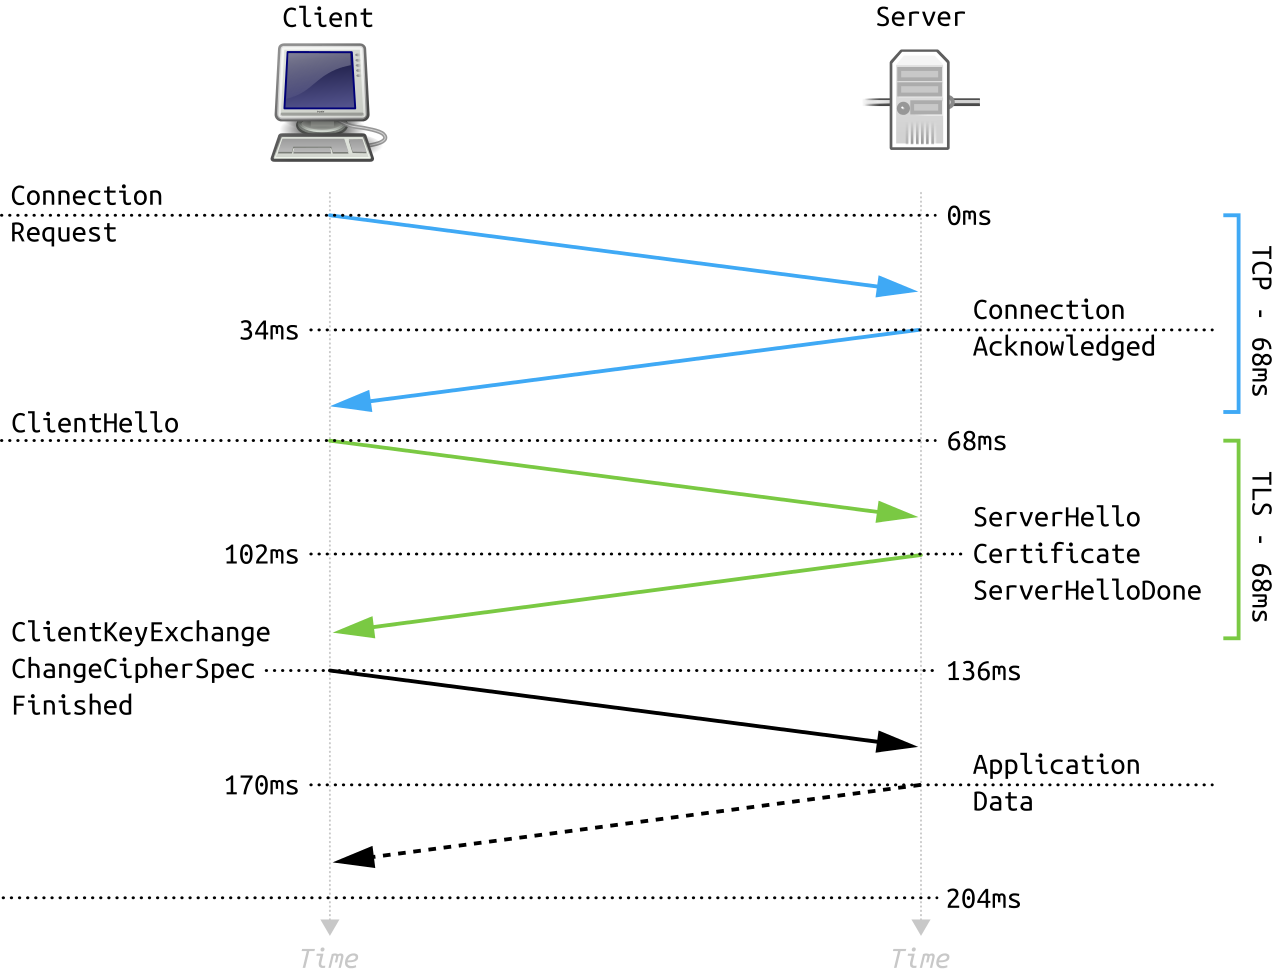
\includegraphics[width=0.7\textwidth]{diagrams/tls_handshake.png}\end{figure}

The above sequence diagram presents the functionality of a TLS handshake.
Client and Server exchange the basic parameters of the connection such as 
the highest TLS protocol version, a random number, a list of suggested cipher 
suites and suggested compression methods. The server provides the client with all
the necessary information in order to validate and use the asymmetric server key, in order
to compute the symmetric key that will be used for the rest of the communication.
The client computes the  PreMasterSecret and sends it to the server 
which is then used by both parties to compute the symmetric key.
Finally, both sides exchange and validate hash and MAC codes over all the
previous messages, after which they both have the ability to communicate safely.

This implies only in the basic TLS handshake. Client-authenticated and resumed handshakes
are quite different, although they are not relevant for the purpose of this work.


\subsection{TLS record}

\begin{figure}[H] \caption{TLS record} \centering
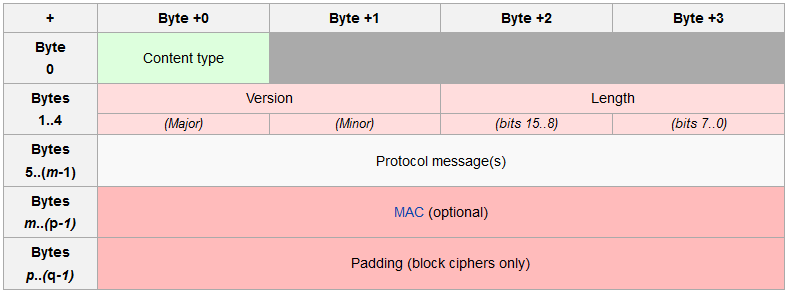
\includegraphics[width=1\textwidth]{diagrams/tls_record.png}\end{figure}

The above figure depicts the general format of all TLS records.

The first field defines the Record Layer Protocol Type of the record, which can
be one of the following:

\begin{table}[H] \centering \begin{tabular}{ | l | l | } \hline \textbf{Hex} &
\textbf{Type} \\ \hline 0x14 & ChangeCipherSpec \\ 0x15 & Alert \\ 0x16 &
Handshake \\ 0x17 & Application \\ 0x18 & Heartbeat \\ \hline \end{tabular}
\end{table}

The second field defines the TLS version for the record message, which is
identified by the major and minor numbers:

\begin{table}[H] \centering \begin{tabular}{ | l | l | l | } \hline
\textbf{Major} & \textbf{Minor} & \textbf{Version} \\ \hline 3 & 0 & SSL 3.0 \\
3 & 1 & TLS 1.0 \\ 3 & 2 & TLS 1.1 \\ 3 & 3 & TLS 1.2 \\ \hline \end{tabular}
\end{table}

The aggregated length of the payload of the record, the MAC and the padding is
then calculated by the following two fields: \begin{math}256*(bits 15..8) +
(bits 7..0)\end{math}.

Finally, the payload of the record, which, depending on the type, may be
encrypted, the MAC, if provided, and the padding, if needed, make up the rest of
the TLS record.

\section{Man-in-the-Middle}\label{sec:mitm}

A man-in-the-middle attack\footnote{\url{https://en.wikipedia.org/wiki/Man-in-the-middle_attack}}
is a type of cyberattack where a malicious actor inserts him/herself into a conversation
between two parties, impersonates both parties and gains access to information that the two 
parties were trying to send to each other. A man-in-the-middle attack allows a malicious actor 
to intercept, send and receive data meant for someone else, or not meant to be sent at all, 
without either outside party knowing until it is too late. 

\begin{figure}[H] \caption{Man-in-the-Middle} \centering
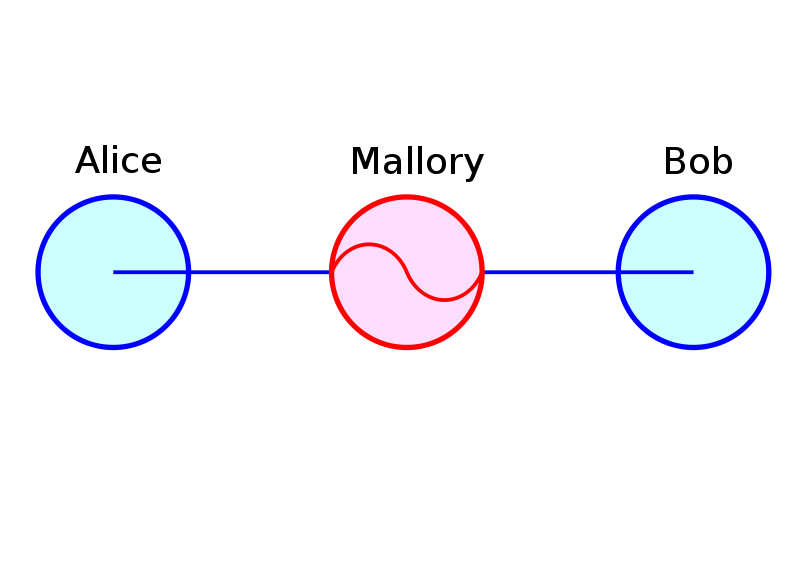
\includegraphics[width=1\textwidth]{diagrams/mitm.png}\end{figure}


MitM attacks can be mitigated using end-to-end encryption, mutual authentication
or PKIs. However, some attacks are still feasible against poorly configured
end-points. Below we describe one such attack, ARP Spoofing.


\subsection{ARP Spoofing}

ARP spoofing is a type of attack in which an attacker sends falsified ARP
(Address Resolution Protocol) messages over a local area network.
This results in the linking of an attacker’s MAC address with the IP address
of a legitimate computer or server on the network. This enables the attacker to
begin receiving any data that is intended for that IP address. ARP spoofing can 
enable malicious parties to intercept, modify or even stop data in-transit.

ARP spoofing can also be used for legitimate reasons, when a developer needs to
debug IP traffic between two hosts. The developer can then act as proxy between
the two hosts, configuring a switch that is used by the two parties to forward
the traffic to the proxy for monitoring purposes.

\begin{figure}[H] \caption{ARP Spoofing} \centering
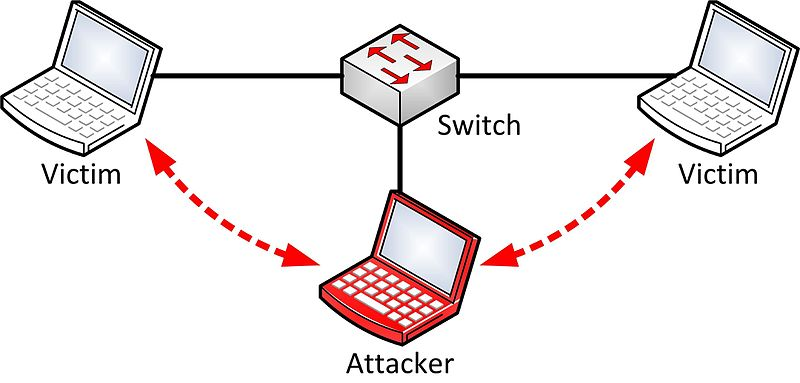
\includegraphics[width=0.8\textwidth]{diagrams/arp_spoofing.jpg}\end{figure}



\chapter{Statistical methods and optimisation techniques}\label{statistic_methods}

Gluck, Harris and Prado in the original BREACH paper investigated the attack on
stream ciphers such as RC4. They also suggested that block ciphers are vulnerable
without providing practical attack details. However, the use of RC4 is prohibited in
negotiation between servers and clients \cite{rc4_prohibit} due to several other major vulnerabili-
ties. 

Block alignment techniques have already been explored in the literature \cite{poodle} and 
Dimitris Karakostas also investigated statistical methods
to attack block ciphers in his thesis.
The section \ref{sec:blockalign} evolves the use of statistical
methods for block cipher attacks in a more structured way.

In the section \ref{sec:optimizations} we also propose various optimization techniques which
make the attack much more efficient.

\section{Block alignment}\label{sec:blockalign}

Block ciphers provide a greater challenge compared to stream ciphers, when it
comes to telling length apart, since stream ciphers provide better granularity. That
is because block ciphers round length to $\lambda$-bits, where $\lambda$ is the block size,
by adding padding.

In order to bypass this, we propose the introdution of artificial noise, 
which will force the creation of additional blocks, if necessary. 
Theoretically, it would be enough to issue $16\times$ more requests
to achieve block alignment. At this point, the correct candidate would result in one less
block, which in turn would provide a measurable length difference. 


\begin{figure}[H] \caption{Block Alginment} \centering
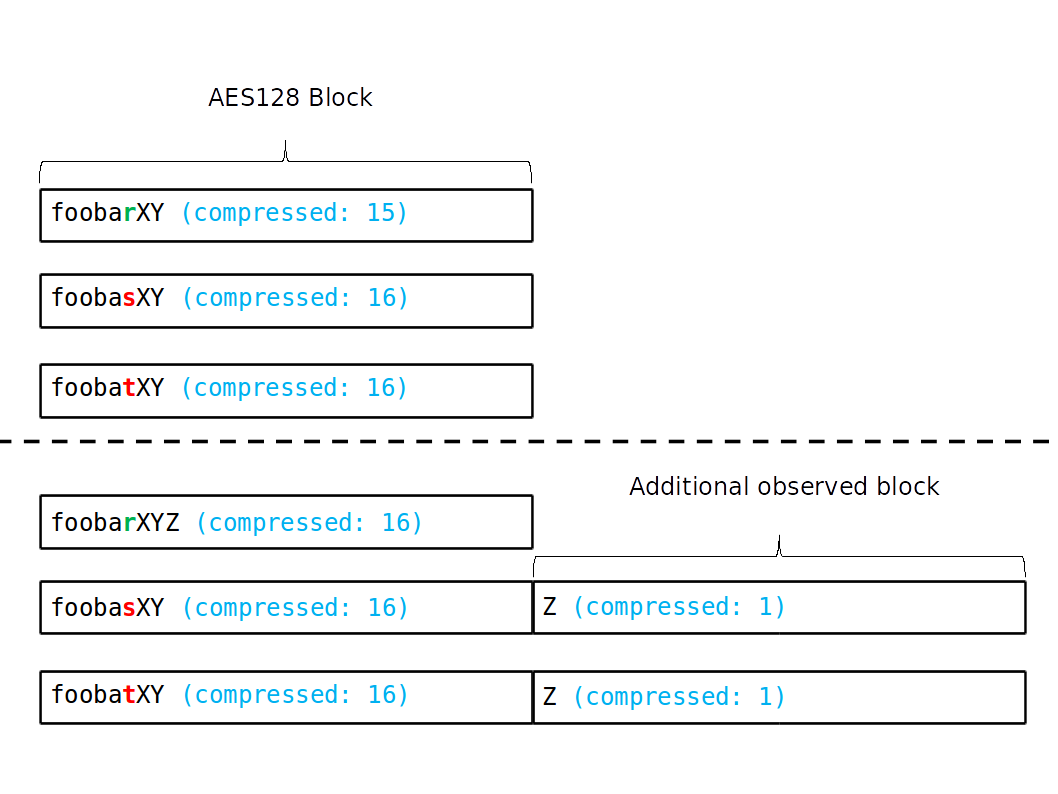
\includegraphics[width=0.7\textwidth]{diagrams/block_alignment.png}\end{figure}

This figure illusrates an example of how the artificial noise results in block alignment and 
how this contributes to distingush between lengths. The example assume a known secret
\textit{fooba} and a possible next byte drawn from the alphabet \textit{(r,s,t)}.
When the attack uses the padding \textit{XY}, the total lenght size 
of the three possible next bytes are the same. Although \textit{foobar} has 15 bits,
they are rounded up to 16 bits in respect of block alginment.
In case of padding \textit{XYZ}, the wrong candidates result in a one more block 
because they cross the block boundaries. Despite the actual difference of only 1 bit,
the use of block ciphers results in 16 bits length difference.


However, introduction of artificial noise is actually tricky. Firstly, noise should be carefully constructed
to avoid being compressed with itself. Secondly, each added symbol will alter the Huffman coding in a
different way, since the plaintext's symbol frequency distribution will be altered. It is advised to use symbols
which do not appear in the rest of the plaintext or they are rare. Even in this casee
 the Huffman tree will be expanded and, consequently, the length of the compressed text will increase,
 in a manner that cannot always be predicted.

\section{Optimizations}\label{sec:optimizations}


\subsection{Request soup}\label{subsec:soup}

A problem with encrypted responses is the fact that it is not possible to safely
determine which packet corresponds to which request, when requests are pipelined
by the browser. That way if the attacker was to issue
requests sequentially, they would have to ensure all response packets for each request
have arrived, before issuing the next one.

However, it is possible to avoid this delay, by making samplesets, each one containing multiple
requests for a specific symbol. For each sampleset, responses would then come pipelined and it
would not be possible to tell them apart. However, this does not indicate a problem since these requests
with the corresponding responses are not adaptive to each other and thus there is no
need to distinguish between then. The total length of the capture can still be
measured and divided by the known amount of requests that the sampleset
contains. This would be enough to calculate the desired mean length.
This statistical mean length converges to the sampleset distribution's mean length due to
the law of large numbers.

This method offers a speedup of up to $5\times$, considering a 200
ms delay and a 40 ms round trip time.



\subsection{Browser parallelization}

The optimization presented in section \ref{subsec:soup} would result in small benefit if no browser
parallelization was possible. Although the attacker would send multiple requests at the same time, the browser
would proceed them pipelined. 

Browsers allow in general up to 6 parallel HTTP requests, although this may differ depending
on the browser application and release. This allows issuing multiple parallel requests and
collecting samples at the same time, giving the attack a $6\times$ speedup.

Each parallel request cannot adapt based on previous results.
However, we need to collect multiple samples per candidate to perform
statistical analysis and extract the mean. These samples pertain to the same
candidate and can be collected non-adaptively.

\begin{figure}[H] \caption{Browser Parallelization} \centering
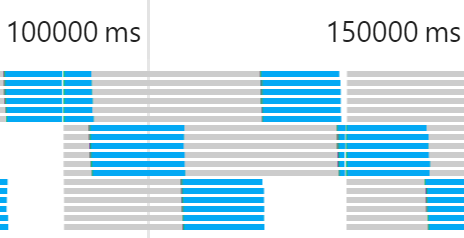
\includegraphics[width=0.7\textwidth]{diagrams/parallel.png}\end{figure}


\chapter{Rupture framework}\label{rupture}

In this chapter, we will describe our framework for conducting compression side-channel attacks,
Rupture. Rupture is a service-based architecture system which contains multiple
independent components.

The section \ref{sec:assumptions} descibes in details the assumptions needed to be made 
in order to orchestrate the attack. The section \ref{sec:principles} describes the 
terminology used in our framework and its governing principles. Finally, the section
\ref{sec:architecture} presents thoroughly the multiple components.
While the components are designed to be able to run
independently on different networks or computer systems, easy instances of the
attack can be performed by running all subsystems on an individual system. We
provide appropriate scripts to conduct such attacks easily.


\section{Attack Assupmtions}\label{sec:assumptions}

The attack framework assumes a \textit{target} service to be attacked. Typically
this target service is a web service which uses TLS. Specifically, we are
targeting services that provide HTTPS end-points. However, this assumption can
be relaxed and attacks against other similar protocols are possible. Any
protocol that exchanges encrypted data on the network and for which a
theoretical attack exists can in principle be attacked using Rupture. We
designed Rupture to be a good playground for experimentation for such new
attacks. Examples of other encrypted protocols for which attacks can be tested
include SMTP and XMPP.

The attack also assumes a user of the target service for which data will be
decrypted, the \textit{victim}. The victim is associated with a particular target.

There are two underlying assumptions in our attack: The injection and the
sniffing assumptions. These are often achieved through the same means, although
not necessarily.

The injection assumption states that the adversary is able to
inject code to the victim's machine for execution. This code is able to issue
adaptive requests to the target service. Injection in Rupture is achieved
through the \textit{injector} component. The code that is injected is the \textit{client}
component.

The sniffing assumption states that the adversary is able to observe network
traffic between the victim and the target. This traffic is typically
ciphertexts. Sniffing is achieved through the \textit{sniffer} component.

Both the referenced \textit{sniffer} and \textit{client} will be presented in section 
\ref{sec:architecture}.



\section{Principles of Attack}\label{sec:principles}


The attack takes place by first injecting client code into the victim's
computer using the injector. The client then opens a command-and-control
channel to the real-time service, which forwards work from the backend to the
client.

When a client associated with a victim asks to work, the backend passes a work
request to the real-time service, which passes it to the client. These work
requests ask the client to perform a series of network requests from the
victim's computer to the target web app. As these requests are made from the
victim's browser, they contain authentication cookies which authenticate the
user to the target service. As such, the responses contain sensitive data, but
that data is not readable by the client due to same-origin policy.

When a response arrives from the target web app to the victim's computer, the
encrypted response is collected by the sniffer on the network. The encrypted
data pertaining to one response is a \textit{sample}. Each work request asks for
multiple requests to be made, and therefore multiple samples are collected per
work request. The set of samples collected for a particular work request are a
\textit{sampleset}.

A successful attack completely decrypts a portion of the plaintext. The portion
of the plaintext which the attack tries to decrypt is the \textit{secret}. That
portion is identified through an initially known prefix which distinguishes it
from other secrets. This prefix is typically 3 to 5 bytes long. Each byte of
the secret can be drawn from a given \textit{alphabet}, the secret's alphabet. For
example, some secrets only contain numbers, and so their alphabet is the set of
numbers [0-9].

At each stage of the attack, a prefix of the secret is known, because that
portion of the secret has already been successfully decrypted. The prefix
decrypted grows until the whole secret becomes known, at which stage the attack
is completed.

When a certain prefix of the secret is known, the next byte of the secret must
be determined. The attack initially assumes the next unknown byte of the secret
can come from the secret's alphabet, but slowly drills down and rejects
alphabet symbols until only one candidate symbol remains. At each stage of the
attack of one byte of the secret, there is a certain **known alphabet** which
the next byte can take. This known alphabet is a subset of the secret's
alphabet.

To drill down on the known alphabet, one of two methods is employed. In the
\textit{serial method}, each symbol of the known alphabet is tried sequentially. In
the \textit{divide \& conquer method}, the alphabet is split into two \textit{candidate
alphabet} subsets which are tried independently.

The attack is conducted in \textit{rounds}. In each round, a decision is made
about the state of the attack and more becomes known about the secret. In a
round, either the next byte of the secret becomes known, or the known alphabet
is drilled down to a smaller set. In order to compare various different
candidate alphabets, the attack executes a series of \textit{batches} of data
collection for each round.

In each batch, several samples are collected from each probability distribution
pertaining to a candidate alphabet, forming a sampleset. When samplesets of the
same amount of samples each have been collected for all the candidate
alphabets, a batch is completed and the data is analyzed. The analysis is
performed by the **analyzer** which statistically compares the samples of
different distributions and decides which distribution is optimal, i.e.
contains the correct guess. This decision is made with some \textit{confidence},
which is expressed in bytes. If the confidence is insufficient, an additional
batch of samplesets is collected, and the analysis is redone until the
confidence value surpases a given threshold.

Once enough batches have been collected for a decision to be made with good
confidence, the round of the attack is completed and more information about the
secret becomes known. Each round at best collects one bit of information of the
secret.

\section{Architecture}\label{sec:architecture}


\subsection{Injector}
The injector component is responsible for injecting code to the victim's
computer for execution. In our implementation, we assume the adversary controls
some network of the victim. Our injector injects the client code in all
unauthenticated HTTP responses that the victim receives. This Javascript code
is then executed by the victim's browser in the context of the respective
domain name. We use bettercap \cite{bettercap}  to perform the HTTP
injection. The injection is performed by ARP spoofing the local network and
forwarding all traffic in a Man-in-the-Middle manner. It is simply a series of
shell scripts that use the appropriate bettercap modules to perform the attack.

As all HTTP responses are infected, this provides increased robustness.
The injected client code remains dormant until it is asked to wake
up by the command-and-control channel. This means that the user can switch
between browsers, reboot their computer, close and reopen browser tabs, and the
attack will keep running.

The injector component needs to run on the victim's network and as such is
light-weight and stateless. It can be easily deployed on a machine such as a
Raspberry Pi, and can be used for massive attacks, for example at public
unencrypted networks such as coffee shops or airports. Multiple injectors can
be deployed to different networks, all controlled by the same central
command-and-control channel.

While injection is performed on the local network through altering HTTP
responses in our case, the injector component is independent and can be
replaced by alternative means. Other good points of injection that can be used
instead of our build-in injector are giving a link directly to the victim via a
phishing mail, in which case attack robustness is limited, or by injecting code
at the ISP or router level if the adversary has such a level of access.


\begin{figure}[H] \caption{Injector Code} \centering
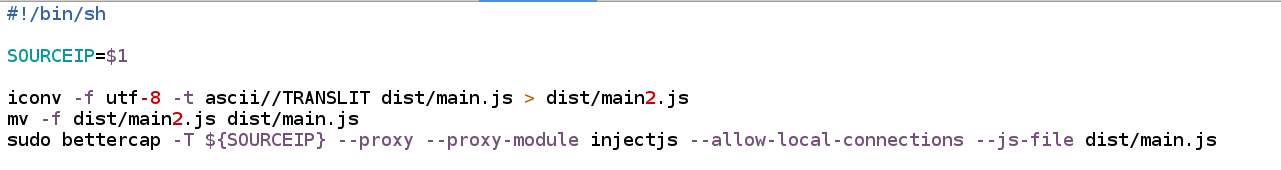
\includegraphics[width=0.7\textwidth]{diagrams/injector.png}\end{figure}


\subsection{Sniffer}

The sniffer component is responsible for collecting data directly from the
victim's network. As the client issues chosen plaintext requests, the sniffer
collects the respective ciphertext requests and ciphertext responses as they
travel on the network. These encrypted data are then transmitted to the backend
for further analysis and decryption.

Our sniffer implementation runs on the same network as the victim. It is a
Python program which uses scapy \cite{scapy} to
collect network data.

Our sniffer runs on the same machine as our injector and utilizes the
injector's ARP spoofing to retrieve the data from the wire or the air. 
Other sniffer alternatives include sniffing data on the target network side, or
on the ISP or router point if the adversary has such a level of access.

The sniffer exposes an HTTP API which is utilized by the backend for
controlling when sniffing starts, when it is completed, and to retrieve the
data that was sniffed. This API is described below.


\subsubsection{backend <-> sniffer (HTTP)}

The Python backend application communicates with the sniffer server, in order
to initiate a new sniffer, get information or delete an existing one. The  sniffer 
server implements a RESTful API for communication with the backend.

\textbf{/start} is a POST request that initializes a new sniffer.
Upon receiving this request, the sniffer service should start sniffing.

The request contains a JSON with the \textit{source\_ip}, 
- the IP of the victim on the local network - and the \textit{destination\_host}
- the hostname of the target that is being attacked.

The backend returns \textit{HTTP 201} if the sniffer is created correctly. Otherwise, it returns
\textit{HTTP 400} if either of the parameters is not properly set, or \textit{HTTP 409 -
Conflict}, if a sniffer for the given arguments already exists.

\textbf{/read} is GET request that asks for the network capture of the sniffer.

The GET parameters are the \textit{source\_ip}  - the IP of the victim on the local network -
and the \textit{destination\_host} - the hostname of the target that is being attacked.

The backend returns \textit{HTTP 200} with a JSON that has a field \textit{capture}, which contains the
network capture of the sniffer as hexadecimal digits, and a field \textit{records},
that contains the total amount of captured TLS application records. In case of
error, \textit{HTTP 422 - Unprocessable Entity} is returned if the captured TLS
records were not properly formed on the sniffed network, or \textit{HTTP 404} if no
sniffer with the given parameters exists.

\textbf{/delete} is a POST request that asks for the deletion of the sniffer

The request contains a JSON with the \textit{source\_ip} - the IP of the victim on the local network - 
and \textit{destination\_host} - the hostname of the target that is being attacked.

The backend Returns \textit{HTTP 200} if the sniffer was deleted successfully, or \textit{HTTP 404} if 
there is no sniffer with the given parameters.

\subsection{Client}

The client runs on the victim machine and is responsible for issuing adaptive
chosen plaintext requests to the target oracle.

The client is written in Javascript and runs in a different context from the
target website. Thus, it is subject to same-origin policy and cannot read the
plaintext or encrypted responses. However, the encrypted requests and responses
are available to the sniffer through direct network access.

The client contains minimal logic. It connects to the real-time service through
a command-and-control channel and registers itself there. Afterwards, it waits
for work instructions by the command-and-control channel, which it executes.
The client does not take any decisions or receive data about the progress of
the attack other than the work it is requested to do. This is intentional so as
to conceal the workings of the adversary analysis mechanisms from the victim in
case the victim attempts to reverse engineer what the adversary is doing.
Furthermore, it allows the system to be upgraded without having to deploy a new
client at the victim's network, which can be a difficult process.

As a regular user is browsing the Internet, multiple clients will be injected
in insecure pages and they will run under various contexts. All of them will
register and maintain an open connection through a command-and-control channel
with the real-time service. The real-time service will enable one of them for
this victim, while keeping the others dormant. The one enabled will then
receive work instructions to perform the required requests. If the enabled
client dies for whatever reason, such as a closed tab, one of the rest of the
clients will be waken up to take over the attack.

The client is a Javascript program written using harmony / ECMAScript 6 and
compiled using babel and webpack.


\subsection{Real-time}

The real-time service is a service which awaits for work requests by clients.
It can handle multiple targets and victims. It receives command-and-control
connections from various clients which can live on different networks,
orchestrates them, and tells them which ones will remain dormant and which ones
will receive work, enabling one client per victim.

The real-time service is developed in Node.js.

The real-time service maintains open web socket command-and-control connections
with clients and connects to the backend service, facilitating the
communication between the two.

The real-time server forwards work requests and responses between the client
and the Django service. The communication it does with the client uses web
sockets in order to achieve bi-directional communication in real-time. This
also facilitates the ability to detect that a client has gone away, which is
registered as a failure to do work. This can happen for example due to network
errors if the victim disconnects from the network, closes their tab or browser,
and so on. It is imperative that incomplete work is marked as failed as soon as
possible so that the attack can continue by recollecting the failed samples.

The web socket API exposed by the real-time service is explained below.

\subsubsection{client <-> real-time protocol}

The client / real-time protocol is implemented using socket.io websockets.

 \textbf{client-hello / server-hello}

When the client initially connects to the real-time server, it sends the message
\textit{client-hello} passing its \textit{victim\_id} to the real-time server.  The server
responds with a \textit{server-hello} message. After these handshake messages are
exchanged, the client and server can exchange futher messages.

 \textbf{get-work / do-work}

When the client is ready to perform work, it emits the message **get-work**
requesting work to be performed from the real-time server. The real-time server
responds with a **do-work** message, passing a *work* object, that is
structured as defined below:

\texttt{
typedef work \\
  amount: int \\
  url: string \\
  timeout: int (ms) \\
}

If the real-time service is unable to retrieve work from the backend due to a
communication error, real-time will return an empty work object indicating
there is no available work to be performed at this time.

 \textbf{work-completed}

When the client has finished its work or has been interrupted due to network
error, it emits a \textit{work-completed} message, containing the following
information:

\texttt
{
  work: work,
  success: bool
}


\textit{success} is \textit{true} if all requests were performed correctly, otherwise it
is \textit{false}. \textit{work} contains the work that was performed or failed to perform.

\subsection{Backend}

The backend is responsible for strategic decision taking, statistical analysis
of samples collected, adaptively advancing the attack, and storing persistent
data about the attacks in progress for future analysis.

The backend talks to the real-time service for pushing work out to clients. It
also speaks to the sniffer for data collection.

It is implemented in Python using the Django framework.

The backend exposes a RESTful API via HTTP to which the real-time service
makes requests for work. This API is explained below.

\subsubsection{real-time -> backend (HTTP)}

The backend implements various API endpoints for communication with the
real-time server.


\textbf{/get\_work/<victim>} is an HTTP GET endpoint. It requests work to 
be performed on behalf of a client. The argument passed is the \textit{victim}
- the id of the victim.

If there is work to be done, it returns an \textit{HTTP 200} response with the JSON
body containing the work structure. The work will contain instructions to
collect multiple samples from the same distribution by performing a series of
similar requests. The samples associated with a particular work request and
performed all together constitute a \textit{sampleset}.

In case no work is available for the client, it returns an HTTP `404` response.
Work can be unavailable in case a different client is already collecting data
for the particular victim, and we do not wish to interfere with it.

\textbf{/work\_completed/<victim>} is an HTTP POST endpoint. It indicates on behalf 
of the client that some work was successfully or unsuccessfully completed. The arguments
passed are the \textit{work} and a boolean \textit{success} parameter

If \textit{success} is \textit{True}, this indicates that the series of indicated requests
were performed by the victim correctly. Otherwise, the victim failed to perform
the required requests due to a network error or a timeout and the work has to
be redone.



\chapter{Rupture API via Web UI}\label{rupture_api}

In this chapter we describe our contributions regarding a RESTful API for Rupture.
We believe that the API enables researchers to fully automate 
TLS-based attacks such as compression side-channel attacks. We
provide a usable, clean set of end-points which can be used to mount the
attack. The RESTful API provides managing targets such as various web services,
victims by robustly injecting and sniffing for information on local networks based on IP
addresses and strategies for advancing attack rounds based on state
search exploration. Is also runs analyses on collected data, which is stored
persistently. We are confident this automation will enable cryptographers and
security researchers to heavily experiment with the various attack parameters,
yielding better attack results in terms of correctness and performance.

\section{RESTful API}
In this section, We describe the implementation of a RESTful API via HTTP 
to which the user makes requests from the web User Interface. This 
RESTful API can also be directly used by programmers without the need 
to use the web interface.

\subsection{/attack}

The \textit{/attack} is an HTTP POST endpoint. 

When the backend receives a POST request, it initiates a new attack.
The arguments passed are the victim's IP and the target. There is also an optional
parameter, the \textit{victim\_id}. If the \textit{victim\_id} is set,
the victim already exists. If no \textit{victim\_id} argument is passed, the backend 
creates and stores a new victim. In both cases, the backend
creates the client and injection code for the specific victim and 
injects the client code to the victim's machine with bettercap. 
It returns \textit{HTTP 200} with a JSON that has a 
field \textit{victimid}, which contains the ID of the new victim.

\subsection{/victim}

The \textit{/victim} is an HTTP POST and GET endpoint. 

When the backend receives a POST request, it creates a new victim. 
The argument passed is the victim's IP. The backend 
creates and stores a new victim, and  returns HTTP 200 with a JSON that has a 
field \textit{victimid}, which contains the ID of the new victim.


On a GET request, the backend returns an HTTP 200 JSON response. 
The JSON contains a list of all the stored victims that the attack 
is still running on or has been completed.

\subsection{/victim/$ <victimId> $}

The /victim/$ <victimId> $ is an HTTP GET, PUT and DELETE endpoint.

On a GET request, the backend returns HTTP 200 with a JSON with details 
for the victim with the specific victimId. The argument passed is the 
victim's Id. The backend returns the general information and details of 
the attack. The general information consists of the victim's IP and 
machine name, the target name, the decrypted secret up to this point 
and a percentage of the progress. Percentage is calculated by dividing the
length of the already decrypted-known secret with the length of the whole secret which 
we want to decrypt. Further details are provided per  batch.
These are the round number, the batch number, the alignment alphabet, 
the possible knownsecret and the confidence.

On a PUT request, the user asks the backend to pause or continue the attack. 
The argument passed is the desired state of the attack, either "paused" 
or "running". The backend updates the current state of the attack and 
returns HTTP 200. 

On a DELETE request, the backend deletes the specific attack.

\subsection{/victim/notstarted}

The \textit{/victim/notstarted} is an HTTP GET endpoint. When a GET request 
is received, the backend scans the wifi network with bettercap to find all 
possible victims and their machine's name. The backend returns a list of 
possible's victims IPs and machine names, which are available on the network
but are not already attacked.


\subsection{/target}
This is an HTTP 200 POST and GET endpoint.
On a POST request, the argument passed to the backend is the name of the target, 
the endpoint, the known prefix, the secret's alphabet, the secret length, 
the alignment alphabet, the records' cardinality and the method of the attack. 
The backend creates and stores the new target and returns HTTP 200 with a JSON 
with the target name.

On a GET request, the backend returns an HTTP 200 JSON response. The JSON contains 
a list of all the stored target for which an attack is possible.



\section{Web UI}                                                                                                          

The user handles the attacks via a web interface which consists 
of two main pages and a modal window. The two main pages are the
\textbf{Network Overview} and the \textbf{Victim Attack Inspection}. 
The modal window is used for the target configuration.

The Network Overview is the start page. It displays the completed,
 the currently running and the paused attacks. It also allows the user 
to initiate a new attack either by adding a custom victim or by scanning 
and choosing one of victims with bettercap.

\begin{figure}[H] \caption{Start Page} \centering
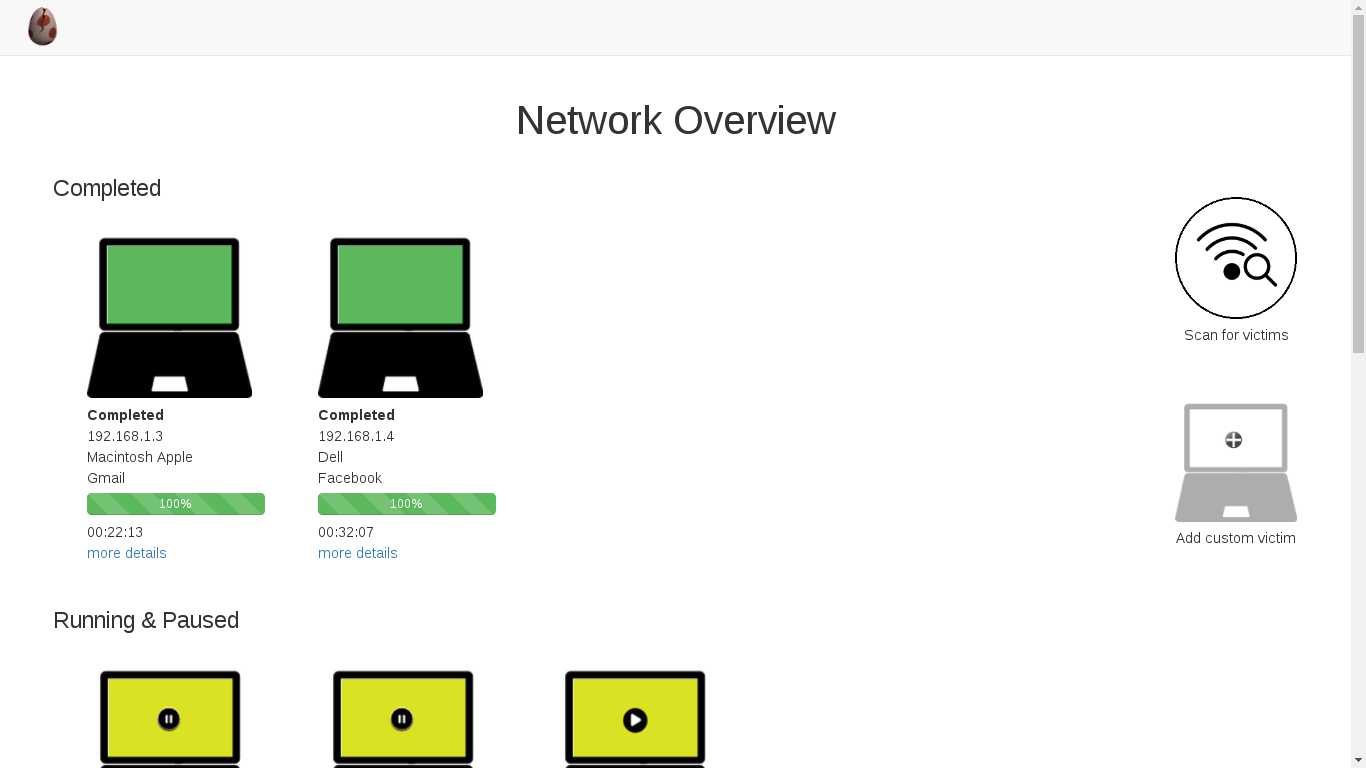
\includegraphics[width=0.7\textwidth]{diagrams/startPage.png}
\end{figure}

The completed and the running or paused attacks are represented by PC icons. 
When the user clicks the \textit{Scan for victims} button, bettercap scans 
the network for possible victims, which are shown beneath the running/paused attacks.
The user can otherwise click on the \textit{Add custom victim} 
button if they already know the victim’s IP and don’t need to search for other victims.

\begin{figure}[H] \centering 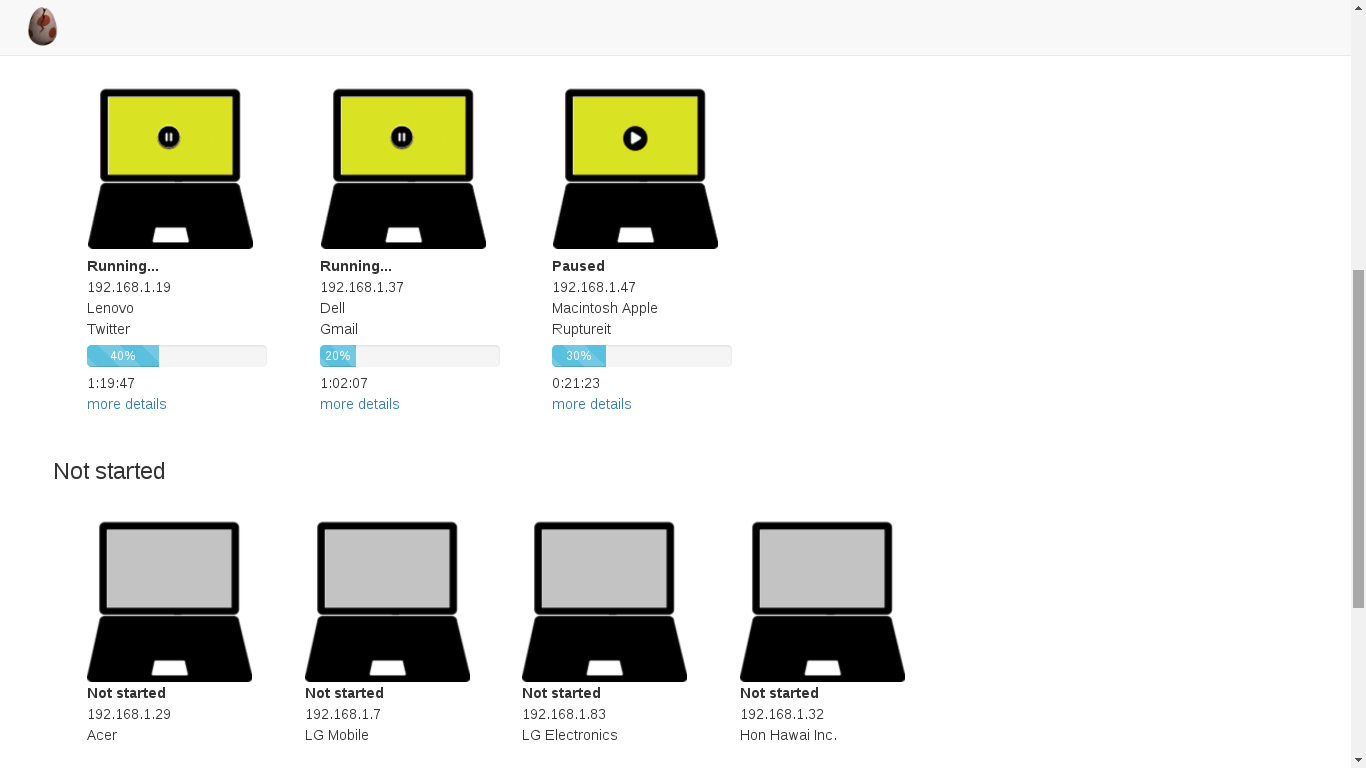
\includegraphics[width=95mm]{diagrams/notstarted.png}
\caption{Possible victims for a new attack} \end{figure}

The victim and target configuration are shown below. If the user has previously scanned 
the network, the victim's IP is already filled.

\begin{figure}[H] \caption{Victim Configuration} \centering 
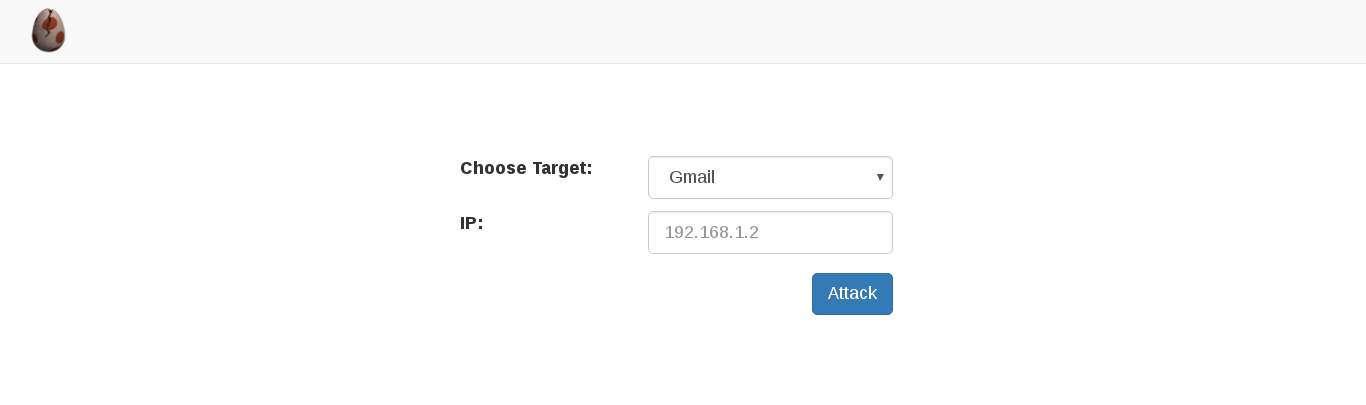
\includegraphics[width=95mm]{diagrams/victim.png} \end{figure}

There are some pre-configured targets but the user can configure a 
new one.


\begin{figure}[H]
    \centering
    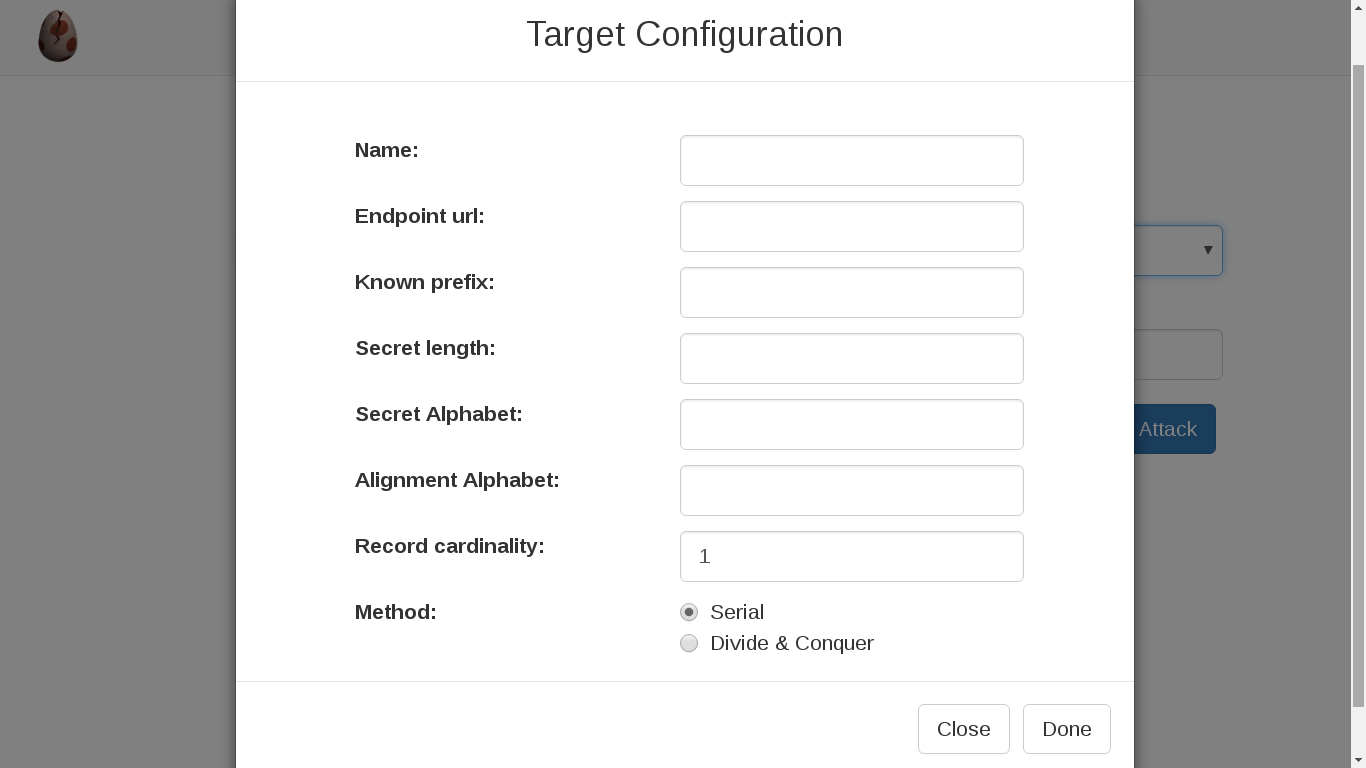
\includegraphics[width=90mm]{diagrams/target.png}
    \caption{Target Configuration}
\end{figure}

When the user clicks on a completed, running or paused attack, 
they can view further details of the attack.

\begin{figure}[H]
    \centering
    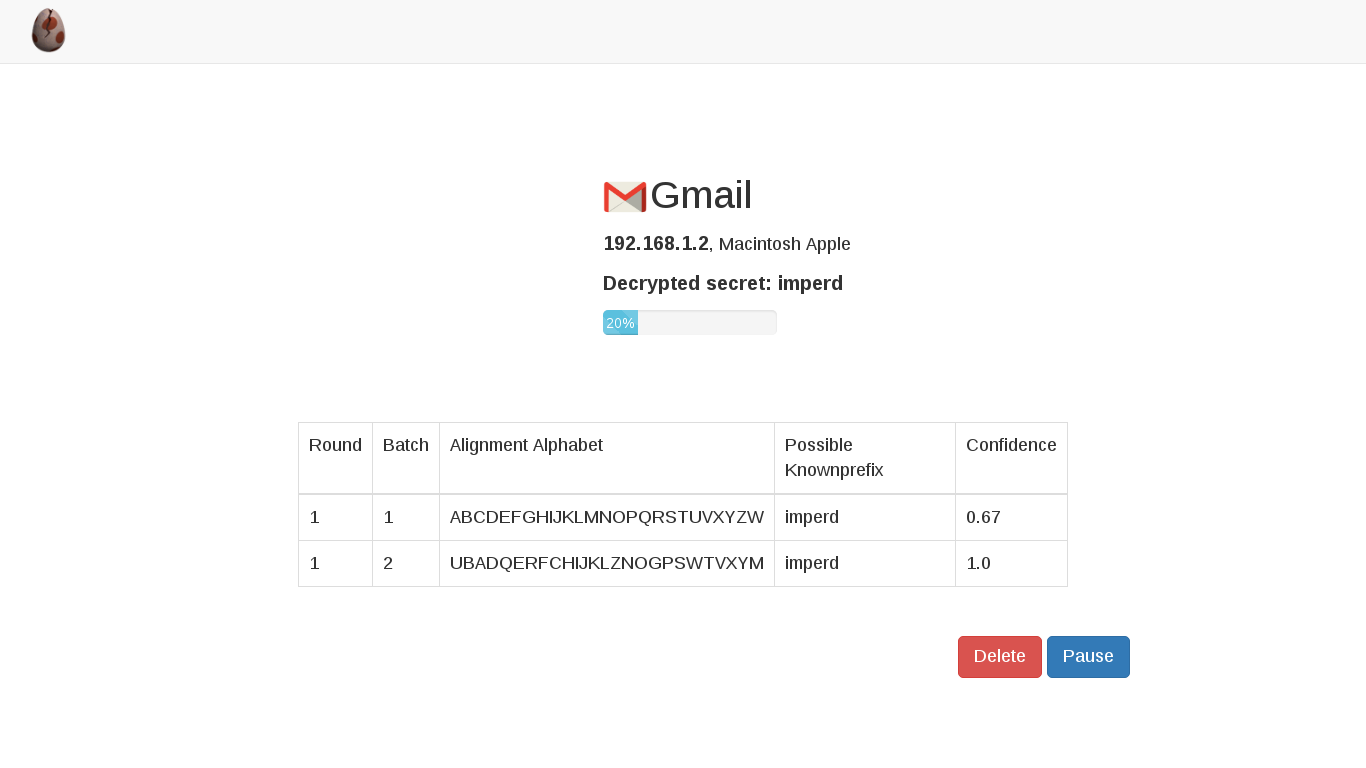
\includegraphics[width=115mm, height=75mm]{diagrams/attack.png}
    \caption{Attack details}
\end{figure}

The above indicate how easily the user can perform the attack in a fully automated way.

\chapter{Appendix}\label{appendix}

\section{Injector}\label{sec:inject.sh}

\plaintext{inject.sh}{inject.sh}                                                                                                  

\section{Client}\label{sec:breach.jsx}

\plaintext{breach.jsx}{breach.jsx}

\section{Sniffer}\label{sec:sniffer.py}

\plaintext{sniffer.py}{sniffer.py}

\section{Real-time}\label{sec:index.js}

\plaintext{index.js}{index.js}

\section{Backend - Strategy}\label{sec:strategy.py}

\plaintext{strategy.py}{strategy.py}

\section{Backend - Analyzer}\label{sec:analyzer.py}

\plaintext{analyzer.py}{analyzer.py}

\section{API views}\label{sec:views.py}

\plaintext{views.py}{views.py}


\bibliography{references}
\bibliographystyle{plain}

\end{document}
